\documentclass[fleqn]{homework}

\student{Stephen Brennan (smb196)}
\course{EECS 440}
\assignment{Written 6}
\duedate{October 6, 2015}

% Solarized colors
%\usepackage[x11names, rgb, html]{xcolor}
\definecolor{sbase03}{HTML}{002B36}
\definecolor{sbase02}{HTML}{073642}
\definecolor{sbase01}{HTML}{586E75}
\definecolor{sbase00}{HTML}{657B83}
\definecolor{sbase0}{HTML}{839496}
\definecolor{sbase1}{HTML}{93A1A1}
\definecolor{sbase2}{HTML}{EEE8D5}
\definecolor{sbase3}{HTML}{FDF6E3}
\definecolor{syellow}{HTML}{B58900}
\definecolor{sorange}{HTML}{CB4B16}
\definecolor{sred}{HTML}{DC322F}
\definecolor{smagenta}{HTML}{D33682}
\definecolor{sviolet}{HTML}{6C71C4}
\definecolor{sblue}{HTML}{268BD2}
\definecolor{scyan}{HTML}{2AA198}
\definecolor{sgreen}{HTML}{859900}

\usepackage{listings}
\lstset{
    % How/what to match
    sensitive=true,
    % Border (above and below)
    frame=lines,
    % Extra margin on line (align with paragraph)
    xleftmargin=\parindent,
    % Put extra space under caption
    belowcaptionskip=1\baselineskip,
    % Colors
    backgroundcolor=\color{sbase3},
    basicstyle=\color{sbase00}\ttfamily,
    keywordstyle=\color{scyan},
    commentstyle=\color{sbase1},
    stringstyle=\color{sblue},
    numberstyle=\color{sviolet},
    identifierstyle=\color{sbase00},
    % Break long lines into multiple lines?
    breaklines=true,
    % Show a character for spaces?
    showstringspaces=false,
    tabsize=2
}

\usepackage{mathtools}
\newcommand{\sigmoid}{\:\text{sigmoid}}

\begin{document}
  \maketitle

  \begin{problem}{1}
    \begin{question}
      Suggest modifications for backpropagation for non-feedforward neural
      network structures: \textbf{(i)} Edges are allowed between nodes in the
      same layer as well as between successive layers, but the graph is still
      directed acyclic. In other words, nodes in layer $k$, $x_{k1}$, $x_{k2}$,
      ..., $x_{kn}$ can have edges between them as well as to the k+1 layer, as
      long as no cycle is created. \textbf{(ii)} Edges are allowed from a layer
      to preceding layers but not into the input layer, so the graph is directed
      cyclic, but the input layer only has outgoing edges. (10 points)
    \end{question}

    \textbf{(i)} So long as there are no cycles, you can go layer by layer, and
    backpropagate the nodes of each layer in an ordering such that each
    successor node is backpropagated before its predecessor.  More generally,
    for any directed acyclic graph, doing backpropagation in the order produced
    by a topological sort will always work.

    \textbf{(ii)} When cycles are introduced, backpropagation can no longer work
    by doing a single pass over the network of nodes.  Instead, you could use an
    iterative approach.  Each iteration, do a pass over every node (probably
    starting at the output layers) computing estimates of the partial
    derivatives.  When you require a partial derivative you haven't computed
    yet, use the previous iteration's estimate (or a random number during the
    first iteration).  Repeat this process until the partial derivative
    estimates for the input layer ``converge'' given some $\epsilon$.
  \end{problem}

  \begin{problem}{2}
    \begin{question}
      Consider a neural network with a single hidden layer with sigmoid
      activation functions and a single output unit also with a sigmoid
      activation, and fixed weights. Show that there exists an equivalent
      network, which computes exactly the same function, where the hidden unit
      activations are the $tanh$ function described in class, and the output
      unit still has a sigmoid activation. (10 points)
    \end{question}

    Consider the hyperbolic tangent function:

    \begin{align*}
      \tanh(u, a, b) &= a\frac{e^{bu} - e^{-bu}}{e^{bu} + e^{-bu}} \\
                     &= a\left(\frac{e^{bu}}{e^{bu}}\right) \frac{e^{bu} - e^{-bu}}{e^{bu} + e^{-bu}} \\
                     &= a\frac{e^{2bu} - 1}{e^{2bu} + 1} \\
                     &= a\frac{e^{2bu} + 1}{e^{2bu} + 1} - a\frac{2}{e^{2bu} + 1} \\
                     &= a - 2 a\frac{1}{1 + e^{2bu}} \\
    \end{align*}

    When $a = b = -\frac{1}{2}$:

    \begin{align*}
      \tanh\left(u, -\frac{1}{2}, -\frac{1}{2}\right)
      &= -\frac{1}{2} + \frac{1}{1 + e^{-u}} \\
      &= -\frac{1}{2} + \sigmoid(u) \\
    \end{align*}

    Using this, we could replace each sigmoid hidden unit with a tanh hidden
    unit where $a = b = -\frac{1}{2}$, whose output will only differ by a
    constant of $-\frac{1}{2}$.  This will cause the input to the output unit's
    sigmoid function to be $w \cdot (-\frac{1}{2} + x)$, which is off by a
    constant value of $-w \cdot (\frac{1}{2}, \frac{1}{2}, ...)$ In order to
    eliminate this difference, we can simply add a dummy input to the output
    unit which is always 1.  We set the weight of that input to
    $(\frac{1}{2}, \frac{1}{2}, \dots) \cdot w$, and the resulting network will
    produce the exact same function as the original network.
  \end{problem}

  \begin{problem}{3}
    \begin{question}
      Draw an artificial neural network structure which can perfectly classify
      the examples shown in the table below. Treat attributes as
      continuous. Show all of the weights on the edges. For this problem, assume
      that the activation functions are sign functions instead of
      sigmoids. Propagate each example through your network and show that the
      classification is indeed correct. (10 points)

      \begin{tabular}{|rr|c|}
        \hline
        $x_1$ & $x_2$ & Class \\
        \hline
        -4 & -4 & - \\
        -1 & -1 & + \\
        1 & 1 & + \\
        4 & 4 & - \\
        \hline
      \end{tabular}
    \end{question}

    My network is shown below.  Weights are labeled next to their edges, and
    $\sigma$ values are labeled above their units.  Since $x_2$ provides no
    additional information, I left it out of my network!
    \begin{center}
      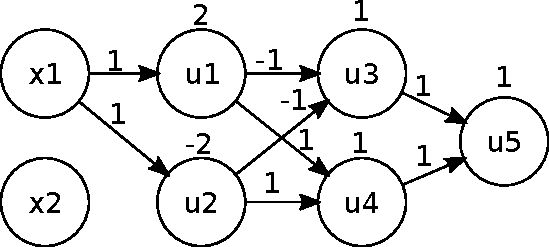
\includegraphics[width=0.6\textwidth]{net.pdf}      
    \end{center}

    Propagated examples: \\

    \begin{tabular}{|rr|rrrrr|}
      \hline
      $x_1$ & $x_2$ & $u_1$ & $u_2$ & $u_3$ & $u_4$ & $u_5$ \\
      \hline
      -4 & -4 & -1 & -1 & 1 & -1 & -1 \\
      -1 & -1 & -1 & 1 & -1 & -1 & 1 \\
      1 & 1 & -1 & 1 & -1 & -1 & 1 \\
      4 & 4 & 1 & 1 & -1 & 1 & -1 \\
      \hline
    \end{tabular}
  \end{problem}

  \begin{problem}{4}
    \begin{question}
      Using R/Matlab/Mathematica/your favorite math software, plot the decision
      boundary for an ANN with two inputs, two hidden units and one output. All
      activation functions are sigmoids.  Each layer is fully connected to the
      next. Assume the inputs range between -5 to 5 and fix all activation
      thresholds to 0. Plot the decision boundaries for the weights except the
      thresholds randomly chosen between \textbf{(i)} $(−10,10)$, \textbf{(ii)}
      $(−3,3)$, \textbf{(iii)} $(−0.1,0.1)$ (one random set for each case is
      enough). Use your plots to show that weight decay can be used to control
      overfitting for ANNs. (If you use Matlab, the following commands might be
      useful: meshgrid and surf). (10 points)
    \end{question}

    \begin{figure}
      \centering
      \caption{Decision boundary for random ANN with weights in (-10, 10).}
      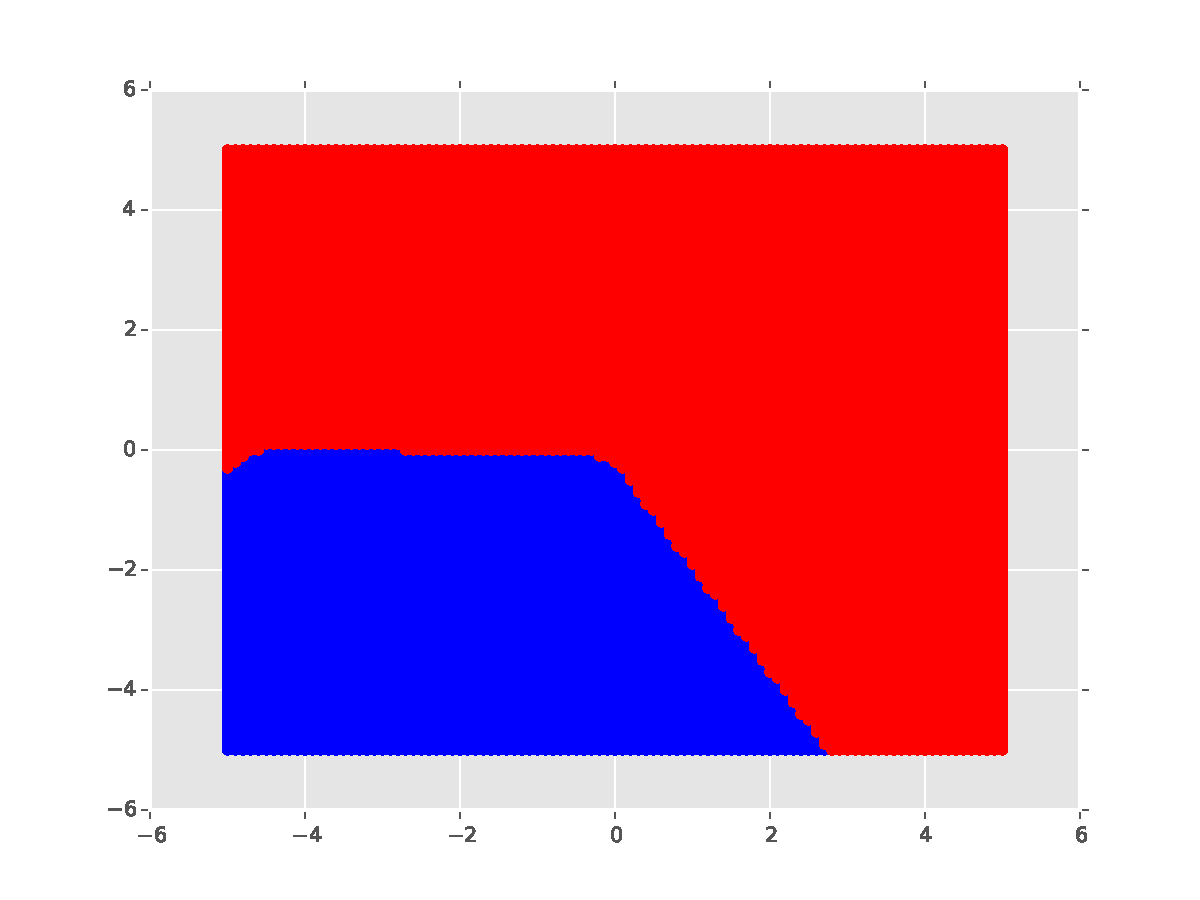
\includegraphics[width=0.7\textwidth]{10.pdf}
      \label{fig:10}
    \end{figure}

    \begin{figure}
      \centering
      \caption{Decision boundary for random ANN with weights in (-3, 3).}
      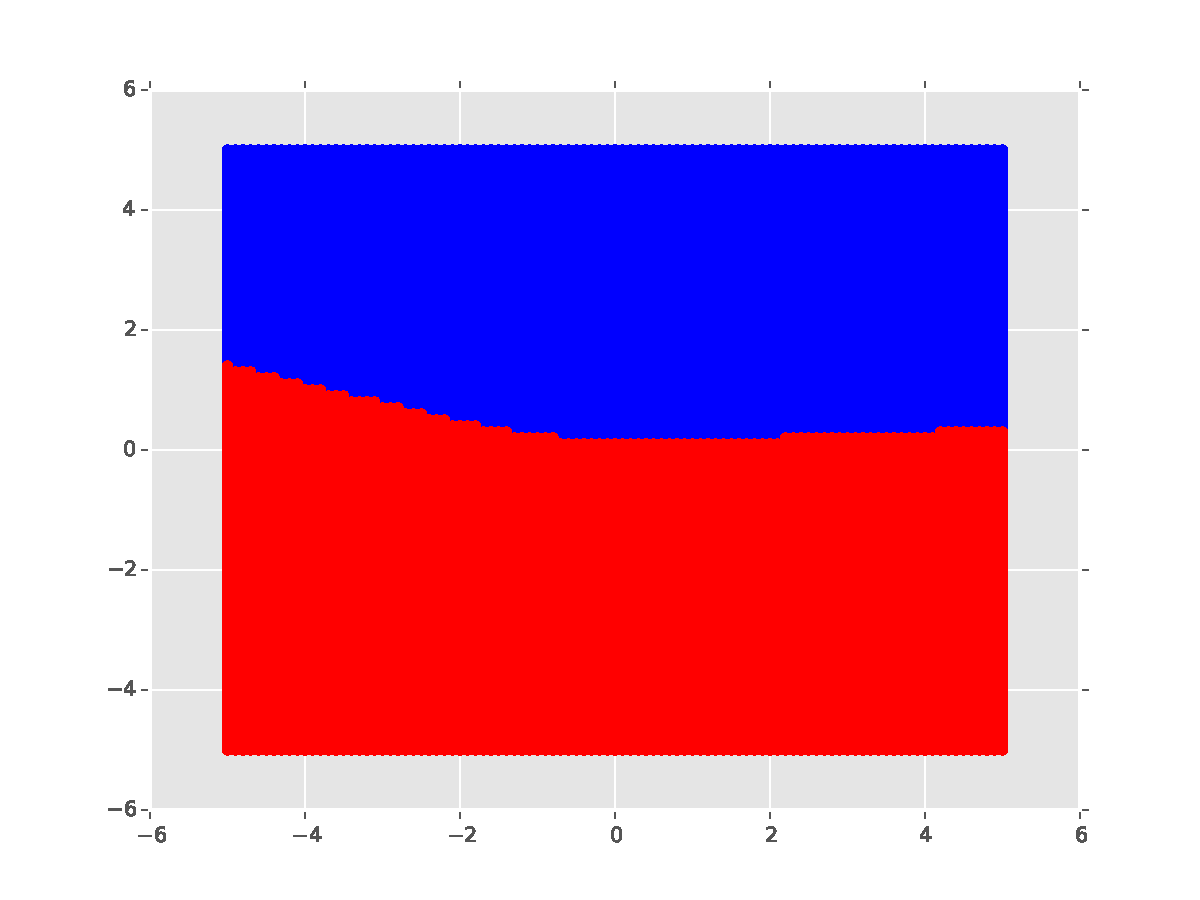
\includegraphics[width=0.7\textwidth]{3.pdf}
      \label{fig:3}
    \end{figure}

    \begin{figure}
      \centering
      \caption{Decision boundary for random ANN with weights in (-0.1, 0.1).}
      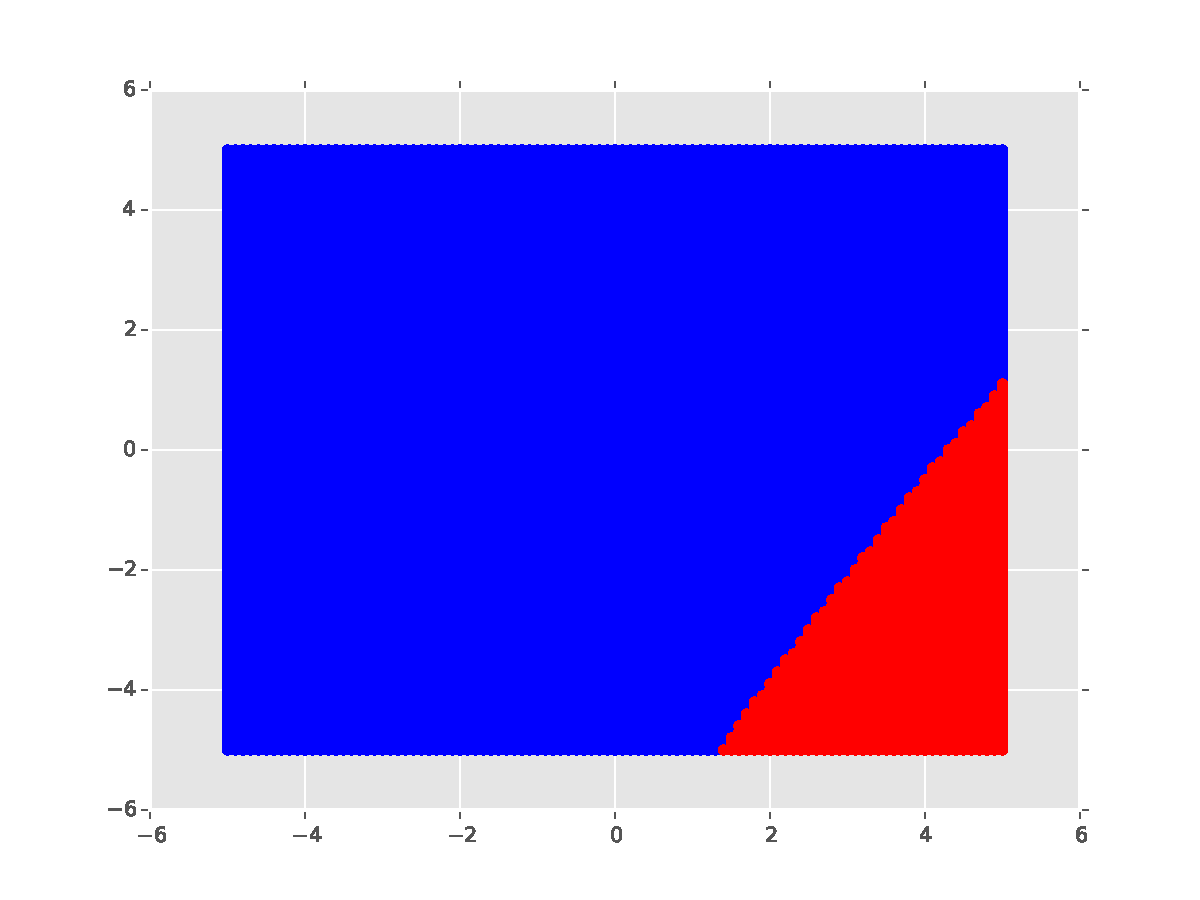
\includegraphics[width=0.7\textwidth]{0_1.pdf}
      \label{fig:0.1}
    \end{figure}

    Plots for \textbf{(i)}, \textbf{(ii)}, and \textbf{(iii)} are provided as
    Figures~\ref{fig:10},~\ref{fig:3}, and~\ref{fig:0.1}, respectively.  In the
    figures, the examples predicted positive are blue, and the examples
    predicted negative are red.  The decision boundary is the boundary between
    the blue and red regions.  You can see that as the weights become closer to
    zero, the decision boundaries become less complex (that is, have fewer
    ``bends'' in them).  Therefore, it stands to reason that creating an
    artificial incentive to have smaller weights would reduce the ``bendiness'',
    and therefore reduce overfitting.

    The Python source code that produced the images is provided in
    Appendix~\ref{p4src}.
  \end{problem}

  \begin{problem}{5}
    \begin{question}
      When learning the weights for the perceptron, we dropped the $sign()$
      activation function to make the objective smooth. Show that the same
      strategy does not work for an arbitrary ANN.  (Hint: consider the shape the
      of decision boundary if we did this.) (10 points)
    \end{question}

    When we train a single perceptron, we drop the $sign()$ function because it
    is not differentiable, and dropping the sign function will give us the same
    result for classification.  However, in an ANN, the output of a unit will be
    used by units in the next layer.  It is important that the activation
    function retains the properties of the $sign()$ function so that these units
    receive consistent input.
  \end{problem}

  \newpage
  \appendix
  \section{Source Code for Problem 4}
  \label{p4src}
  \lstinputlisting[language=Python]{w06.py}

  Example: \texttt{\$ python w06.py 10}
\end{document}